\chapter{Physics}
\label{physics_chap}

This chapter
outlines the physics options available in the {\wrf}. 
The WRF physics options fall into several categories, each containing
several choices. The physics categories are (1) microphysics, 
(2) cumulus parameterization, (3) planetary boundary layer (PBL), 
(4) land-surface model, and (5) radiation. Diffusion, which
may also be considered part of the physics, 
is described in Chapter \ref{filter_chap}. 

The physics section is separated from the dynamics in the solver by the 
use of physics drivers. These drivers are between dynamical-core-dependent parts
of the solver: a  pre-physics preparation of variables and post-physics 
modifications of the tendencies. The physics preparation involves filling
arrays with physics-required variables that include the temperature,
pressure, heights, layer thicknesses,
and other state variables in MKS units at half-level grid points and on full levels.
The velocities are also de-staggered so that the physics part is independent
of the dynamical solver's velocity staggering. Physics packages 
compute tendencies
for the velocity components (un-staggered), potential temperature, and moisture
fields. A post-physics step will re-stagger these tendencies
as necessary, couple tendencies with coordinate metrics, and convert
to variables or units appropriate to the dynamics solver.

In the first Runge-Kutta step, prior to the acoustic steps (see Fig.
\ref{time_integration_figure}, step(1)), tendencies are computed for
radiation, surface, PBL, and cumulus physics. These tendencies
are then held fixed through the Runge-Kutta steps. Microphysics is
computed after the last Runge-Kutta step 
(see Fig. \ref{time_integration_figure},
step (9)) in order to ensure proper saturation conditions at the end 
of the time-step.

The initialization of the physics is
called prior to the first model step. This initialization may include reading
in data files for physics tables or calculating look-up tables of functions.
Each physics module includes an initialization routine for this purpose.
Often physics packages will have many of their own constants that are
included in their own module, while common physical constants are
passed in from the physics drivers.


\section{Microphysics}

Microphysics includes explicitly resolved water vapor, cloud, and 
precipitation processes. The model is general enough to accommodate any 
number of mass mixing-ratio variables, and other quantities
such as number of particles per unit dry air mass. Four-dimensional arrays with three spatial
indices and one species index are used to carry such scalars.
Memory, i.e., the size of the fourth dimension in these
arrays, is allocated depending on the needs of the scheme chosen, 
and advection of the species also applies to all those required 
by the microphysics option. In the current version of ARW, microphysics 
is carried out at the end of the time-step as an adjustment process, 
and so does not provide tendencies but directly updates the state variables. 
The rationale for this is that 
condensation adjustment should be at the end of the time-step
to guarantee that the final saturation balance is accurate for the 
updated temperature and moisture. However, it is also important to 
have the latent heating forcing for potential temperature during the 
dynamical sub-steps, and this is done by saving the microphysical 
heating as an approximation for the next time-step as described in Section
\ref{diabatic forcing subsection}.

Currently, the sedimentation process is accounted for inside the 
individual microphysics modules, 
and, to prevent instability in the calculation of the vertical flux of
precipitation, either a smaller time step is allowed or a Lagrangian scheme is used. 
The saturation adjustment is also 
included inside the microphysics. In the future, however, it might be separated 
into an individual 
subroutine to enable the remaining microphysics to be called less frequently 
than the model's advection step for efficiency.

The various microphysics options have differing
numbers of moisture variables, depending on the ice-phase and mixed-phase
processes included. Mixed-phase processes are those that result from
the interaction of ice and water particles, such as riming that produces
graupel or hail.
As a general rule, for grid sizes less than 10 km, where updrafts may be
resolved, mixed-phase schemes should be used, particularly in convective
or icing situations. For coarser grids it may not be worth the added expense of these schemes
because riming is not likely to occur with the relatively weak vertical motion that is resolved.
Many schemes are also double-moment for some species and include
number per unit dry air mass for those as extra advected variables.

\subsection{Kessler scheme}

This scheme \citep{kessler69}, which was taken from the COMMAS model
\citep{wicker95}, is a simple 
warm cloud scheme that includes water vapor, cloud water, and rain. 
The microphysical processes included are: the production, fall, and 
evaporation of rain; the accretion and autoconversion of cloud water;
and the production of cloud water from condensation.

\subsection{Purdue Lin scheme}

Six classes of moisture variables are included: water vapor, cloud water, rain, cloud ice, 
snow, and graupel. All parameterization production terms are based on \citet{lin83}
and \citet{rutledge84} with some modifications, including condensation 
adjustment with saturation assumptions following \citet{tao89} and ice sedimentation. Compared to Kessler, the
treatment of ice processes in this and all the other microphysics options increases 
the level of sophistication, and makes it more generally suitable for use 
in research studies. The scheme is taken from the Purdue cloud model, and 
the details can be found in \citet{chen02}.

\subsection{WRF Single-Moment 3-class (WSM3) scheme}

The WRF single-moment 3-class microphysics scheme follows \citet{hong04} including ice sedimentation and other new ice-phase parameterizations. A major difference from other approaches is that a diagnostic relation is used for ice number that is based on ice mass content rather than temperature. The computational procedures are described in \citet{honglim06}. As with WSM5 and WSM6, the fall terms are computed using a Lagrangian technique instead of time-splitting that was used in earlier versions of these schemes. The WSM3 scheme predicts three categories of moist variables: water vapor, cloud water/ice, and rain/snow, making it a so-called simple-ice scheme. It follows \citet{dudhia89} in assuming cloud water and rain for temperatures above freezing, and cloud ice and snow for temperatures below freezing. This scheme is computationally efficient for the inclusion of ice processes, but lacks supercooled water and gradual melting rates. 

\subsection{WSM5 scheme}

This scheme is similar to the WSM3 simple ice scheme. However, water vapor, rain, snow, cloud ice,
and cloud water are held in five different arrays. Note that the numbering of these schemes includes water vapor as a class which is different from other
numbering conventions. Thus, it allows supercooled water to exist, and
a gradual melting of snow falling below the melting layer. Details can be found in 
\citet{hong04}, and \citet{honglim06}. As with WSM6, the saturation adjustment follows \citet{dudhia89} and \citet{hong98} in separately treating ice and water saturation processes, rather than a combined saturation such as the Purdue Lin (above) and Goddard \citep{tao89} schemes. This scheme is efficient in intermediate grids between the mesoscale and cloud-resolving grids.

\subsection{WSM6 scheme}

The six-class scheme extends the WSM5 scheme to include graupel and its associated processes.
Some of the graupel-related terms follow \citet{lin83}, but its ice-phase behavior is much different due to the changes of \citet{hong04}. A new method is introduced for representing mixed-phase particle fall speeds for the snow and graupel particles by assigning a single fallspeed to both that is weighted by the mixing ratios, and applying that fallspeed to both sedimentation and accretion processes \citep{dudhia08}. The behavior of the WSM3, WSM5, and WSM6 schemes differ little for coarser mesoscale grids, but they work differently on cloud-resolving grids. Of the three WSM schemes, the WSM6 scheme is the most suitable for cloud-resolving grids, considering the efficiency and theoretical backgrounds \citep{honglim06}. All of the WSM and WDM schemes compute effective radii for ice, snow and cloud water to interact with RRTMG radiation. All except WSM3 compute reflectivity diagnostics.

\subsection{WDM5 and WDM6 schemes}

These schemes have the same ice-phase processes as WSM5 and WSM6, but warm-rain processes are now double-moment calculations \citep{lim10} with number for cloud and rain being calculated as prognostic variables. The schemes are therefore also sensitive to cloud-condensation nuclei (CCNs) numbers that are also advected, but these are initialized with a constant value. As with all the WSM schemes, sedimentation is handled with a Lagrangian scheme. Also as with WSM5 and WSM6, the method of \citet{dudhia08} is used
to provide a combined fallspeed for snow and graupel.

\subsection{WSM7 and WDM7 schemes}

The extension of WSM6 and WDM6 to include hail as a separate category from graupel is also available as a choice in WRF as WSM7 and WDM7 respectively \citep{bae18}. 
These schemes, by allowing for hail, also can give more intense precipitation rates. As with the other WDM schemes, WDM7 only affects the cloud and rain water processes.

\subsection{Eta Grid-scale Cloud and Precipitation (2001) scheme}

This is also known as EGCP01 or the Eta Ferrier scheme. The scheme predicts changes 
in water vapor and condensate in the forms of cloud water, rain, cloud 
ice, and precipitation ice (snow/graupel/sleet).  The individual hydrometeor 
fields are combined into total condensate, and it is the water vapor 
and total condensate that are advected in the model. 
Local storage arrays retain first-guess information that extract 
contributions of cloud water, rain, cloud ice, and precipitation ice of 
variable density in the form of snow, graupel, or sleet. The density of 
precipitation ice is estimated from a local array that stores information 
on the total growth of ice by vapor deposition and accretion of liquid water. 
Sedimentation is treated by partitioning the time-averaged flux of 
precipitation into a grid box between local storage in the box and 
fall out through the bottom of the box. This approach, together with 
modifications in the treatment of rapid microphysical processes, permits 
large time steps to be used with stable results. The mean size of 
precipitation ice is assumed to be a function of temperature following 
the observational results of \citet{ryan96}. Mixed-phase processes are 
now considered at temperatures warmer than -30$^\circ$C (previously 
-10$^\circ$C), 
whereas ice saturation 
is assumed for cloudy conditions at colder temperatures. Further 
description of the scheme can be found in Sec. 3.1 of the November 
2001 Technical Procedures Bulletin (TPB). 
An advection option has been added for this scheme that explicitly advects cloud water, rain and ice
and includes a rimed fraction.

\subsection{Thompson et al. and aerosol-aware Thompson-Eidhammer schemes}
This is a bulk microphysics scheme that has double-moment ice and rain and has been updated as described by \citet{thompson08}. The aerosol-aware scheme \citep{thompson14}
additionally has prognostic variables for ice-friendly and water-friendly nuclei that are initialized from a global monthly climatology based on aerosols. The scheme has been developed for midlatitude convective, orographic and snowfall conditions especially at convection-permitting grid scales. It is used operationally in the RAP/HRRR forecasting system. The ice, snow,
and cloud droplet radii are passed to the RRTMG radiation schemes along with the clear-sky aerosols for optical depth calculations. Reflectivity is also diagnosed.

\subsection{Goddard Cumulus Ensemble Model scheme}

The Goddard Cumulus Ensemble (GCE) models \citep{tao93} one-moment bulk microphysical schemes  are mainly based on \citet{lin83} with additional processes from \citet{rutledge84}.  However, the Goddard microphysics schemes have several modifications. 

First, there is an option to choose either graupel or hail as the third class of ice in the so-called 3ICE scheme \citep{mccumber91}.  Graupel has a relatively low density and a high intercept value (i.e., more numerous small particles).  In contrast, hail has a relative high density and a low intercept value (i.e., more numerous large particles).  These differences can affect not only the description of the hydrometeor population and formation of the anvil-stratiform region but also the relative importance of the microphysical-dynamical-radiative processes. 

Second, new saturation techniques \citep{tao89, tao03} were added.  These saturation techniques are basically designed to ensure that super saturation (sub-saturation) cannot exist at a grid point that is clear (cloudy).  

Third, all microphysical processes that do not involve melting, evaporation or sublimation (i.e., transfer rates from one type of hydrometeor to another) are calculated based on one thermodynamic state.  This ensures that all of these processes are treated equally. 

Fourth, the sum of all sink processes associated with one species will not exceed its mass.  This ensures that the water budget will be balanced in the microphysical calculations .

The Goddard microphysics has a simpler option, which is equivalent to a two-ice (2ICE) scheme having only cloud ice and snow.  This option may be sufficient for coarse resolution simulations (i.e., $>$ 10 km grid size).  The two-class ice scheme could be applied for winter and frontal convection.

\subsection {Goddard 4ICE  scheme}

The new Goddard 4ICE scheme \citep{lang14, tao16} is a significant improvement over the previous Goddard 3ICE WRF scheme.  The new 4ICE scheme explicitly predicts the evolution of hail in addition to the traditional ice, snow, and graupel categories available in the 3ICE scheme.  The 4ICE scheme was built upon improved versions of the Goddard 3ICE scheme developed for the Goddard Cumulus Ensemble model and includes dozens of new/modified functions regarding ice microphysics and unique particle-size mapping and observation-driven snow density.

\subsection {Morrison et al. 2-Moment scheme}

The \citet{morrison08} scheme is based on the two-moment bulk
microphysics scheme of \citet{morrison05} and \citet{morrison06}. Five species of
hydrometeor are included with water vapor: cloud droplets, cloud ice, rain, snow, and
graupel/hail. The code has a user-specified switch to include either graupel or hail. 
Prognostic variables include number and mass mixing ratios
of cloud ice, rain, snow, and graupel/hail, and mixing ratios of cloud
droplets and water vapor (total of 10 variables). The prediction of two-moments (i.e., both number and mass
mixing ratio) allows for a more robust treatment of the particle size
distributions, which are a key for calculating the microphysical process rates
and cloud/precipitation evolution. Several liquid, ice, and mixed-phase
processes are included. Particle size distributions are treated using gamma
functions, with the associated intercept and slope parameters derived from the
predicted mixing ratio and number.
The scheme has been extensively tested and compared with both
idealized and real case studies covering a wide range of conditions.

\subsection {Milbrandt-Yau Double-Moment scheme}
The \citet{milbrandt05} scheme is a fully double-moment scheme that carries graupel and hail as separate species.
It therefore has 12 prognostic variables in addition to water vapor.

\subsection {CAM Morrison-Gettelman scheme}
The \citet{morrisongettelman08} scheme matches the microphysics used in the CESM CAM5.1 climate model. It is added as part of the CAM
suite of physics. It carries cloud water, ice, rain and snow as double-moment prognostic variables. It is primarily designed for global low resolution applications.

\subsection {Stony-Brook University Lin-Colle scheme}
A single-moment bulk microphysics scheme \citep{lin11} that predicts cloud water, rain, ice and snow and also carries riming intensity
to represent graupel densities.

\subsection {NSSL microphysics schemes}
There are multiple National Severe Storms Laboratory (NSSL) options by \citet{mansell10} ranging from single-moment with graupel
properties specified \citep{gilmore04} or predicted with hail added to double-moment of all species with or without hail and also optionally adding CCNs.

\subsection {HUJI spectral bin microphysics schemes}
The Hebrew University of Jerusalem, Israel, (HUJI) spectral bin microphysics (SBM) scheme has ``fast" and  ``full" versions.
Both resolve size distributions into 33 mass-doubling size bins for each type of particle. The fast scheme \citep{khain10} has four
particle types cloud/rain, ice/snow, graupel and aerosols, while the full scheme \citep{khain04} has eight types cloud/rain, snow, graupel, aerosols,
ice plates, columns and dendrites and hail. The aerosols are cloud condensation nuclei. Note that each bin variable is advected
making these schemes computationally an order of magnitude more costly than bulk microphysics options. Also cloud-resolving to LES
scales are required to represent the details of motion and supersaturation that such schemes require.

\subsection {Predicted Particle Properties (P3) scheme}
The P3 scheme \citep{morrison15} uses a novel approach for predicting properties of ice particles as they transition to
snow and may rime into graupel. The scheme has double-moment rain with an option for double-moment cloud to
handle aerosol effects. The ice is also double-moment, but also has associated scalars for rimed mass and volume that
allow the ice-particle properties to evolve rather than imposing categories like snow, graupel and hail.

\subsection {Jensen ISHMAEL microphysics}
The ISHMAEL (Ice-Spheroids Habit Model with Aspect-ratio EvoLution) scheme \citep{jensen17} can predict ice-particle habits
that are defined by their aspect ratios and volumes and how these develop through deposition and riming. Up to three independent
habits are carried which contain generalized particles that represent the whole evolution from ice to snow to graupel together with their numbers
per unit dry air mass.


\section{Cumulus Parameterization}

These schemes are responsible for the sub-grid-scale effects of 
convective and/or shallow clouds. The schemes are intended to 
represent vertical fluxes due to unresolved updrafts and 
downdrafts and compensating motion outside the clouds. They 
operate only on individual columns where the scheme is triggered and 
provide vertical heating and moistening profiles. Some schemes 
additionally provide cloud and precipitation field tendencies 
in the column, and some provide momentum tendencies 
due to convective transport of momentum. The schemes all provide 
the convective component of surface rainfall.

Cumulus parameterizations are theoretically only valid for coarser grid sizes,
(e.g., greater than 10 km), where they are necessary to properly
release convective available potential energy on a realistic time scale in the convective grid columns.
While the assumptions about the convective eddies being entirely
sub-grid-scale break down for finer grid sizes, sometimes these
schemes have been found to be helpful in triggering convection in
5--10 km grid applications. Generally, they should not be used when
the model can resolve the deep convective updrafts itself (e.g., $\le$ 4 km grid).

A few schemes have developed capability to adapt to finer grid sizes. As the grid sizes
decrease, these schemes will reduce the effect of deep convection accordingly, or gradually turn
off deep convection and let the shallow convection take over.

Note that some cumulus schemes include both deep and shallow
convection, while others only include deep convection.
  
\subsection{Kain-Fritsch schemes}

\subsubsection{Modified Kain-Fritsch Scheme}
The modified version of the Kain-Fritsch scheme \citep{kain04} is based on 
\citet{kain90} and \citet{kain93}, but has been modified based on 
testing within the Eta model. As with the original KF scheme, 
it utilizes a simple cloud model with moist updrafts and downdrafts, 
including the effects of detrainment, entrainment, and relatively 
simple microphysics. It differs from the original KF scheme in the following ways:

\begin{itemize}\setlength{\parskip}{-4pt}
\item
 A minimum entrainment rate is imposed to suppress widespread convection 
in marginally unstable, relatively dry environments.

\item
Shallow (non precipitating) convection is allowed for any updraft 
that does not reach minimum cloud depth for precipitating clouds; 
this minimum depth varies as a function of cloud-base temperature.

\item
The entrainment rate is allowed to vary as a function of low-level convergence.

\item
Downdraft changes:

\begin{itemize}\setlength{\parskip}{-4pt}
\item
Source layer is the entire 150 -- 200 mb deep layer just above cloud base.

\item
Mass flux is specified as a fraction of updraft mass flux at cloud base.
Fraction is a function of source layer RH rather than wind shear 
or other parameters, i.e., old precipitation efficiency relationship not used.

\item
Detrainment is specified to occur in updraft source layer and below.
\end{itemize}

\item
A new way to compute perturbation temperature added to the testing updraft 
parcel is implemented based on \citet{ma2009}. This perturbation temperature
is a function of horizontal and vertical moisture advection, rather than vertical
velocity. This changes the trigger function in the original scheme to work better
in a weakly forced environment.

\item
Subgrid cloud fraction due to both deep and shallow convection is estimated and passed
to the radiation schemes \citep{alapaty12}.
\end{itemize}

\subsubsection{Multi-Scale Kain-Fritsch Scheme}

This is based on the original Kain-Fritsch scheme, and modified to allow 
the scheme to adapt when the grid-size decreases from the mesoscale range (a few tenths 
of kilometers) to convective scales (a few kilometers) \citep{zheng16}. The main modification includes 
a dynamic adjustment time scale for CAPE removal, a modified scale-dependent minimum 
entrainment rate, and an enhanced grid-scale vertical motion using subgrid scale updraft 
mass fluxes. The scheme also includes an option to interact with climatological 
aerosol through an addition of subgrid-scale cloud microphysics \citep{glotfelty19}.

\subsubsection{Kain-Fritsch Cumulus Potential Scheme}

In this version of the Kain-Fritsch scheme, the trigger function in the original scheme 
is replaced by a method that relates the initiation of convection to the distribution of 
temperature and moisture in the boundary layer via probability density functions (PDFs)
\citep{berg13}. The scheme has tunable 
parameters to set for the critical cumulative frequency of bins in order to trigger deep 
convection, and minimum frequency of a bin within the PDF required to form shallow convection. 
The scheme also computes the cumulus cloud fraction due to shallow convection and feeds it into 
the radiation physics. In addition, the scheme can include vertical transport of trace gases and 
aerosols, aqueous chemistry, wet removal and aerosol effect on cloud drop number when 
activated with the MOSAIC chemistry \citep{berg15}.


\subsection{Betts-Miller-Janjic scheme}

The Betts-Miller-Janjic (BMJ) scheme  \citep{janjic94,janjic00} 
was derived from the Betts-Miller (BM) convective adjustment scheme 
\citep{betts86,bettsmiller86}.  However, the BMJ scheme differs 
from the Betts-Miller scheme in several important aspects. The deep convection 
profiles and the relaxation time are variable and depend on the cloud 
efficiency, a non-dimensional parameter that characterizes the convective 
regime \citep{janjic94}. The cloud efficiency depends on the entropy change, 
precipitation, and mean temperature of the cloud. The shallow convection 
moisture profile is derived from the requirement that the entropy change be 
small and nonnegative \citep{janjic94}.  The BMJ scheme has been optimized 
over years of operational application at NCEP,
so that, in addition to the described conceptual 
differences, many details and/or parameter values differ from those 
recommended in \citet{betts86} and \citet{bettsmiller86}.  Recently, attempts 
have been made to refine the scheme for higher horizontal resolutions, 
primarily through modifications of the triggering mechanism.  In particular:
 
\begin{itemize}\setlength{\parskip}{-4pt}
\item
A floor value for the entropy change in the cloud is set up below which the 
deep convection is not triggered;
\item
In searching for the cloud top, the ascending parcel mixes with the environment; and
\item
The work of the buoyancy force on the ascending parcel is required to exceed 
a prescribed positive threshold.
\end{itemize}

\subsection{Grell Schemes}

\subsubsection{Grell-Devenyi Ensemble Scheme}

\citet{grell02} introduced an ensemble cumulus scheme 
in which effectively multiple cumulus schemes and variants are run 
within each grid box and then the results are averaged to give the 
feedback to the model. In principle, the averaging can be weighted 
to optimize the scheme, but the default is an equal weight. 
The schemes are all mass-flux type schemes, but with differing updraft 
and downdraft entrainment and detrainment parameters, and precipitation 
efficiencies. These differences in static control are combined with 
differences in dynamic control, which is the method of determining 
cloud mass flux. The dynamic control closures are based on convective 
available potential energy (CAPE or cloud work function), low-level 
vertical velocity, or moisture convergence. Those based on CAPE 
either balance the rate of change of CAPE or relax the CAPE to a 
climatological value, or remove the CAPE in a convective time scale. 
The moisture convergence closure balances the cloud rainfall to the 
integrated vertical advection of moisture. Another control
is the trigger, where the maximum cap strength that permits convection
can be varied. These controls typically provide ensembles of 144 members.

\subsubsection{Grell-3 Scheme}

The Grell-3 scheme was first introduced in Version 3.0. It shares a lot in
common with the Grell-Devenyi in scheme, being based on an ensemble mean
approach, but the quasi-equilibrium approach is no longer included
among the ensemble members. The scheme is distinguished from other
cumulus schemes by allowing subsidence effects to be spread to
neighboring grid columns, making the method more suitable to grid sizes
less than 10 km, while it can also be used at larger grid sizes where
subsidence occurs within the same grid column as the updraft. 

\subsubsection{Grell-Freitas Scheme}

The Grell-Freitas scheme \citep{grell14} is based on Grell-Devenyi 
scheme which considers a stochastic approach to cumulus convection, and modified 
to work across grid-sizes from mesoscale to convective scales. The scheme 
relates the convective updraft fraction to the entrainment rate, 
which in turn is related the cloud radius. As the grid size decreases, the 
fractional updraft area increases, which is equivalent to decreasing 
the unit mass flux required to stabilize the atmosphere.

\subsection{Simplified Arakawa-Schubert Schemes}

This group of schemes is based on simplified Arakawa-Schubert scheme (SAS) \citep{grell93} 
which considers only one type of cloud instead of an ensemble. They all use the 
quasi-equilibrium closure. They vary by how they handle convective downdrafts, 
shallow convection, momentum transport (all three not included in the original 
AS and last two not in SAS), entrainment/detrainment and scale-aware aspects.

\subsubsection{Original SAS Scheme}

This is the convective scheme used by GFS from 1995 to 2000 \citep{pan95}. This version 
includes a moist convective downdraft, has a shallow component that uses an 
eddy diffusion approach, and considers convective momentum transport which 
depends on vertical wind shear. However the convective momentum transport 
was not implemented in ARW. 

\subsubsection{New SAS Scheme}

The so-called NSAS scheme is an updated SAS scheme operational in GFS since July 2010 \citep{han11}. In this version, 
the shallow convection using an eddy diffusion approach is replaced by a mass-flux 
scheme similarly formulated to deep convection, with entrainment/detrainment 
following LES studies. The deep convection is made stronger by removing random 
cloud-top selection and increasing the maximum allowable mass-flux at the cloud base. 
The entrainment and detrainment are modified to be dependent on environmental relative 
humidity as in the new Tiedtke scheme. The trigger function is modified to have some 
dependency on large-scale vertical velocity and subcloud layer environmental moisture. 
The scheme uses a similar convective momentum transport formulation, but with a reduced effect.

\subsubsection{Scale-aware SAS Scheme}

This variation of the SAS scheme is based on NSAS, but with scale-aware features added. 
The fractional area occupied by the deep convection increases based on updraft radius 
which is in turn dependent on entrainment. This is similar to the assumption used by 
the Grell-Freitas scheme, but using the actual entrainment rate at cloud base. This scheme 
is currently employed in Hurricane WRF.

\subsubsection{KIAPS Scale-aware SAS Scheme}

This is another variation of the updated NCEP SAS scheme from 2010, 
with an added scale-aware dependency \citep{kwon17}. The scale-awareness is implemented by considering 
the fractional updraft area to increase as the grid size decreases. Two factors determine 
the increase: one is empirical and the other is dependent on the ratio of grid vertical 
velocity over convective updraft velocity. In addition to mass-flux dependency on the grid size, 
the convective inhibition and convective cloud water detrainment are also made to depend on grid size.
Note that this is a deep-only scheme and designed to be run with the separate shallow
NSAS cumulus scheme.

\subsection{Zhang-McFarlane Scheme}

The Zhang-McFarlane scheme is a mass-flux scheme and it is only for deep convection \citep{zhang95}. 
It follows the ideas of Arakawa-Schubert, but makes simplified 
assumptions. One of the assumptions is that instead of using a spectrum of cloud plumes, 
it specifies the distribution of the updraft assuming that they all have the same cloud 
base mass flux, but each has a characteristic entrainment rate. It also assumes that the 
convection removes CAPE at an exponential rate with a specified adjustment time scale. 
The scheme detrains cloud liquid and ice, and considers momentum transport. The scheme 
is ported from CAM4, and tested with other CAM physics. For example, it can be 
used together with Park-Bretherton shallow convection option and CAM microphysics.

\subsection{Tiedtke Schemes}

There are two versions of the original Tiedtke scheme \citep{tiedtke89} in ARW. The first version is based on an earlier version 
of the scheme from ECMWF, and the newer version is closer to the code in recent IFS by ECMWF.

\subsubsection{Tiedtke Scheme}

The Tiedtke scheme is a mass-flux scheme, and it parameterizes deep, 
shallow and midlevel convection. It represents the cloud ensemble by a bulk cloud model, 
and considers entrainment and detrainment and downdrafts. It uses a CAPE closure to 
determine the strength of the deep and midlevel convection, and surface evaporation 
for shallow convection. In the version implemented in WRF \citep{zhangc11}, turbulent 
entrainment and detrainment are added and turbulent entrainment for shallow convection 
is increased to promote boundary layer cloud formation. Another modification is to change 
how detrained cloud at the top is treated: in the original scheme, it evaporates immediately; 
and in the current scheme, it is added to the grid scale. To limit the deep convection in 
drier regions, a minimum relative humidity of 80\% is imposed for the mean RH between cloud base and top.

\subsubsection{New Tiedtke Scheme}

This is an updated version of Tiedtke scheme, and it is closer to the one used in the 
recent ECMWF IFS \citep{zhangc17}. The updates include trigger functions for deep and shallow convection, 
closures for deep and shallow convection, convective adjustment time scale, entrainment 
and detrainment rates for all types of convection, conversion from cloud water/ice to 
rain/snow and options for momentum transport. The entrainment for deep convection is 
made to depend on environmental moisture which helps the simulated tropical systems. 
The updated CAPE closure for deep convection relaxes to CAPE generated in the planetary 
boundary layer which improves the diurnal precipitation over land. The convective 
adjustment time is no longer a constant, but it depends on the vertical velocity averaged 
in the updraft and cloud depth.


\section{Shallow Cumulus Parameterization}

Similar to the deep cumulus parameterization, these schemes represent the sub-grid-scale transport of heat 
and moisture in shallow, and sometimes non-precipitating, clouds. Since the scale of shallow convective
cloud is generally smaller than its deep counterpart, it should be used in models when a deep cumulus
scheme is turned off. These stand-alone shallow schemes can therefore serve that purpose. 

\subsection{University of Washington Scheme}

The University of Washington shallow convection scheme is a mass flux scheme \citep{park09} using moist 
adiabatically conserved variables of total specific humidity and liquid water potential 
temperature. The scheme allows for precipitation, considers momentum mixing, and an entrainment 
formulation that depends on the vertical velocity of the updraft. The scheme's closure is 
controlled by convective inhibition. This scheme is adopted from CAM4.

\subsection{GRIMs Scheme}

The GRIMs (The Global and Regional Integrated Model System) shallow convection scheme \citep{hong18} is based 
on the shallow convection scheme of Tiedtke and uses an eddy-diffusivity method. The modification 
to the Tiedtke scheme includes defining the cloud base at the top of the PBL and diffusion 
coefficient as a function of relative humidity, mixed-layer vertical velocity scale and the 
entrainment depth at the PBL top. The scheme is non-precipitating and can only be used with YSU PBL scheme.

\subsection{NSAS Scheme}

This shallow convection scheme is the same as the shallow component in the NSAS scheme.

\subsection{Deng Scheme}

The Deng scheme \citep{deng03} is a mass flux scheme. It considers both buoyant updraft and cloud with nearly neutral buoyancy.
The scheme triggers convection based on the turbulent kinetic energy (TKE) in the boundary layer, and its closure uses a
hybrid formulation that depends on both boundary layer TKE as well as CAPE.
In conditionally unstable environment, the scheme transitions to the Kain-Fritsch deep convective scheme.
The scheme also predicts cloud fraction and cloud liquid content from the detrained convective updraft air.

\section{Surface Layer}

The surface layer schemes calculate friction velocities and exchange 
coefficients that enable the calculation of surface heat and moisture 
fluxes by the land-surface models and surface stress in the planetary 
boundary layer scheme. Over water surfaces, the surface fluxes and surface 
diagnostic fields are computed in the surface layer scheme itself. The schemes 
provide no tendencies, only the stability-dependent information about 
the surface layer for the land-surface and PBL schemes.
Currently, each surface layer option is tied to particular boundary-layer
options, but in the future more interchangeability and options may become
available. Note that some boundary layer schemes (ACM2 and MRF) require
the thickness of the surface layer in the model to be representative of the
actual surface layer (e.g. 50-100 meters) while most others can have thin surface
layers. The schemes use Monin-Obukhov similarity theory with variations in
the stability functions and methods for computing roughness lengths.
Similarity theory relates the information at the lowest model level to the
surface via a stability dependent, approximately log, profile of wind and
scalars. Diagnostic outputs of 2m and 10m quantities are consistently
computed with the profiles of these schemes.

\subsection{Revised MM5 similarity theory}

\citet{jimenez12} revised the previous MM5 similarity theory by improving the
consistency between Ri and z/L and removing limits by using new stability
functions for stable and unstable conditions that also include the extra term
$\psi(z_0/L)$. The scheme gives largely similar results to the old option but shows
some improvement in the transition periods. Both the MM5-based schemes
have the same thermal roughness length options in addition to convective velocity.
The thermal roughness length allows for a reduced roughness length in 
the calculation of $\theta_*$ while the convective velocity adds to $u_*$
for the purposes of scalar fluxes but not friction. Over the ocean, options
for tropical cyclones include a Donelan-based formulation for wave
roughness and a Garratt formulation or constant $z_{0q}$ for enthalpy fluxes.

\subsection{Similarity theory (MYJ/Eta)}

The Eta surface layer scheme \citep{janjic96,janjic02} is based 
on similarity theory \citep{monin54}. The scheme 
includes parameterizations of a viscous sub-layer. Over water surfaces, the 
viscous sub-layer is parameterized explicitly following \citet{janjic94}. 
Over land, the effects of the viscous sub-layer are taken into account 
through variable roughness height for temperature and humidity as proposed by 
\citet{zilit95}. The \citet{beljaars94} correction is applied in order 
to avoid singularities in the case of an unstable surface layer and vanishing 
wind speed. The surface fluxes are computed by an iterative method. 
This surface layer scheme must be run in conjunction with the Eta
(Mellor-Yamada-Janjic) PBL scheme, and is therefore sometimes referred to
as the MYJ surface scheme.

\subsection{QNSE similarity theory}

This should be used with the Quasi-Normal Scale Elimination (QNSE) PBL scheme
\citep{sukoriansky05} named for a theoretical technique employed to derive sub-grid
mixing properties of stratified turbulence. The theory provides effective viscosity and
diffusivity as a function of Richardson number that are used in the stable PBL regime
and the surface layer similarity functions for stable conditions. The scheme is also
distinguished by have a Prandtl number of 0.7 instead of a value near 1. 

\subsection{MYNN surface layer}

The MYNN surface-layer scheme includes  several forms for stability functions with \citet{dyer70}
used by default. There are also several options for handling thermal roughness lengths and the 
fluxes over water. It is to be used with the MYNN PBL options that is part of the RAP/HRRR physics
suite.

\subsection{Similarity theory (PX)}

The PX surface layer scheme \citep{pleim06} was developed as part of the PX LSM but can be used with any LSM or PBL model.  This scheme is based on similarity theory and includes parameterizations of a viscous sub-layer in the form of a quasi-laminar boundary layer resistance accounting for differences in the diffusivity of heat, water vapor, and trace chemical species.   The surface layer similarity functions are estimated by analytical approximations from state variables.  

\subsection{TEMF surface layer}

This surface layer scheme is designed to work with the Total Energy Mass Flux (TEMF) PBL scheme
\citep{angevine10}. The similarity functions used in this scheme are functions of Ri for stable conditions,
and consider unstable conditions similarly to neutral conditions.

\subsection{Similarity theory (MM5) -- old version}

This scheme is now superseded by the Revised MM5 similarity theory scheme
(see above) but still available as an option.
This scheme uses stability functions from \citet{paulson70}, \citet{dyer70}, 
and \citet{webb70}
to compute surface exchange coefficients for heat, moisture, and momentum. 
A convective velocity following \citet{beljaars94} is used to enhance surface 
fluxes of heat and moisture. A Charnock relation relates 
roughness length to friction velocity over water. There are four stability 
regimes following \citet{zhanganthes82}.
This surface layer scheme must be run in conjunction with the MRF or
YSU PBL schemes. Since Version 3, there has been an option to replace the Charnock
relation for roughness length with a Donelan relation that has lower
drag at hurricane-force wind speeds, and may be more suitable for hurricane
simulations. Also for water points, the Beljaars formulation for convective
velocity is replaced by one proportional only to the vertical thermal gradient
to help in weak-wind situations.



\section{Land-Surface Model and Other Surface Options}

The land-surface models (LSMs) use atmospheric information from the surface layer scheme, 
radiative forcing from the radiation scheme, and precipitation forcing from the 
microphysics and convective schemes, together with internal information on the 
land's state variables and land-surface properties, to provide heat and moisture 
fluxes over land points and sea-ice points. These fluxes provide a lower boundary 
condition for the vertical transport done in the PBL schemes (or the vertical 
diffusion scheme in the case where a PBL scheme is not run, such as in 
large-eddy mode). The land-surface 
models have various degrees of sophistication in dealing with thermal and moisture 
fluxes in multiple layers of the soil and also may handle vegetation, root, and 
canopy effects and surface snow-cover prediction. The land-surface model provides 
no tendencies, but does update the land's state variables which include the ground (skin) 
temperature, soil temperature profile, soil moisture profile, snow cover, and 
possibly canopy properties. There is no horizontal interaction between neighboring
points in the LSM, so it can be regarded as a one-dimensional column model for
each WRF land grid-point.

\subsection{5-layer thermal diffusion}

This simple LSM is based on the MM5 5-layer soil temperature model. Layers are 
1, 2, 4, 8, and 16 cm thick. Below these layers, the temperature is fixed at a
deep-layer average. The energy budget includes radiation, sensible, and 
latent heat flux. It also allows for a snow-cover flag, but the snow 
cover is fixed in time. Soil moisture is also fixed with a landuse- and 
season-dependent constant value, and there are no explicit vegetation effects.

\subsection{Noah LSM}

The Noah LSM is the successor to the OSU LSM described by \citet{chendudhia01}. 
The scheme was developed jointly by NCAR and NCEP, and is a unified
code for research and operational purposes, being almost identical
to the code used in the NCEP North American Mesoscale Model (NAM). This has the benefit of 
being consistent with the time-dependent soil fields provided in the analysis datasets.
This is a 4-layer soil temperature and moisture model with canopy 
moisture and snow cover prediction. The layer thicknesses are 10, 30, 60 and 100 cm
(adding to 2 meters) from the top down. It includes root zone, evapotranspiration,
soil drainage, and runoff, taking into account vegetation categories,
monthly vegetation fraction, and soil texture. The scheme provides sensible and latent 
heat fluxes to the boundary-layer scheme. The Noah LSM additionally predicts 
soil ice, and fractional snow cover effects, is linked to urban model options,
and considers surface emissivity properties, which are all new since the OSU
scheme. There is a sub-tiling (mosaic) option for this LSM \citep{li13} that allows
fractional areas of different land-use categories within a grid cell.

\subsection{NoahMP LSM}

This model follows on from the Noah LSM and is a large collaborative effort \citep{niu11, yang11} to allow for multiple parameterization options
for each part of the LSM physics making it a multi-parameterization (MP) scheme. The sub-options within this scheme
include dynamic vegetation, stomatal resistance, runoff/groundwater, soil permeability, radiative transfer, soil and snow
options and surface evaporation resistance options. The scheme has 4 soil layers and 3 snow layers.
There are also a crop model options. NoahMP is linked to all the urban options like Noah (UCM, BEP and BEM).

\subsection{Rapid Update Cycle (RUC) Model LSM}

The RUC LSM has a multi-level soil model (6 levels is default, could be 9 or more) with higher resolution in the top part of soil domain 
(0, 5, 20, 40, 160, 300 cm is default). The soil model solves heat diffusion and Richards moisture transfer equations, and in the cold season
takes into account phase changes of soil water \citep{smirnova97, smirnova00}. 
The RUC LSM also has a multi-layer snow model with changing snow density, refreezing liquid water 
percolating through the snow pack, snow depth and temperature dependent albedo, melting algorithms applied at both 
snow-atmosphere interface and snow-soil interface, and simple parameterization of fractional snow cover with possibility of 
grid averaged skin temperature going above freezing. It also includes vegetation effects and canopy water.
The RUC LSM has a layer approach to the solution of energy and moisture budgets. 
The layer spans the ground surface and includes half of the first atmospheric layer and half of the top soil layer with the 
corresponding properties (density, heat capacity, etc.) The residual of the incoming fluxes (net radiation, latent and sensible heat fluxes, 
soil heat flux, precipitation contribution into heat storage, etc.) modifies the heat storage of this layer. 
An implicit technique is applied to the solution of these equations.
Prognostic variables include soil temperature, volumetric liquid, frozen and total soil moisture contents, 
surface and sub-surface runoff, canopy moisture, evapotranspiration, latent, sensible and soil heat fluxes, 
heat of snow-water phase change, skin temperature, snow depth and density, and snow temperature. 
This option also has a sub-grid mosaic sub-option to allow for fractional areas of different land-use categories.

\subsection{Pleim-Xiu LSM}

The PX LSM \citep{pleim95, xiu01}, originally based on the ISBA model of \citet{noilhan89}, includes a 2-layer force-restore soil temperature and moisture model.  The top layer is taken to be 1 cm thick, and the lower layer is 99 cm. The PX LSM features three pathways for moisture fluxes: evapotranspiration, soil evaporation, and evaporation from wet canopies.  Evapotranspiration is controlled by bulk stomatal resistance that is dependent on root zone soil moisture, photosynthetically active radiation, air temperature, and the relative humidity at the leaf surface.   Grid aggregate vegetation and soil parameters are derived from fractional coverages of land use categories and soil texture types.  There are two indirect nudging schemes that correct biases in 2-m air temperature and RH by dynamic adjustment of soil moisture \citep{pleim03} and deep soil temperature \citep{pleim08}.  Note that a small utility program (ipxwrf) can be used to propagate soil moisture and temperature between consecutive runs to create a continuous simulation of these quantities. The scheme also
allows for sub-grid variability by averaging grid-cell properties from sub-grid fractions.

\subsection{Community Land Model (CLM4)}

CLM4 is a version of the land component of the Coupled Earth System Model (CESM) that is used for climate modeling \citep{oleson10, lawrence11}. 
The model has 10 soil layers and 5 snow layers.
The scheme allows for sub-grid tiling by 5 main categories (glacier, wetland, vegetated, lake and urban), and 4 vegetated sub-tiles of different ``plant functional types" (PFTs).
This has a rather comprehensive set of physics related to land-surface, soil, hydrology, and vegetation processes, also including urban areas, glaciers, and a multi-layer lake
model that is also an option to run with other LSMs in WRF.

\subsection{Simplified Simple Biosphere Model (SSiB)}

SSiB \citep{xue91, sun01}, the LSM from the UCLA GCM as another climate option for land-surface physics. It has a 2-layer bulk soil temperature model,
vegetation effects at the surface, 3 layers of soil moisture with a root zone, and a 4-layer snow treatment. It also predicts canopy temperature and moisture.

\subsection{Urban Canopy Model}

This can be run as an option with the Noah and NoahMP LSMs.
In order to represent the city scale effects on the mesoscale,
an urban canopy model (UCM) originally developed by \citet{kusaka01}
and \citet{kusaka04} and later on modified
by \citet{chen06}, is coupled to the WRF model via
Noah Land surface model. In the UCM, all the urban effects in the
vertical are assumed to be subgrid scale meaning that the urban
processes are occurring below the lowest model level. The urban
canopy model includes:
\begin{itemize}\setlength{\parskip}{-4pt}
\item Parameterization of street canyons to represent the urban
geometry
\item  Shadowing from building and radiation reflection
\item  An exponential wind profile in the canopy layer
\item A multilayer heat equation for roof, wall and road surfaces
\end{itemize}

The urban canopy model estimates the surface temperature and heat
fluxes from the roof, wall and road surface. It also calculates
the momentum exchange between the urban surface and the atmosphere.
If they are available, the UCM can take three different densities
of urban development using special land-use categories.
Since Version 3, an anthropogenic heating diurnal cycle has been added as
an option.

\subsection{Building Environment Parameterization (BEP)}

This is an urban option that also aims to account for more of the dynamical effects of buildings on the flow \citep{martilli02}.
The option is available for the Noah and NoahMP LSMs.
The buildings are allowed to directly impact more than the lowest model layer with suitable choices of PBL schemes (MYJ and Bougeault-Lacarrere).
The scheme is also adaptable to more detailed urban morphology datasets such as NUDAPT and WUDAPT.

\subsection{Building Energy Model (BEM)}

An urban option that builds on BEP to include a building energy budget including heat transfer through walls, windows, floors, roofs, etc., and effects of air conditioning
in controlled environments and other anthropogenic internal heating
in addition to the external urban canyon representations that exist in other urban schemes \citep{salamanca10}. This model allows for a prediction of energy consumption.
This option is also available with the Noah and NoahMP LSMs.

\subsection{Ocean Mixed-Layer Model}

This can be selected as an independent option for water surfaces, and is designed for
hurricane modeling in order to simulate the cooling of the ocean underneath
hurricanes. The ocean mixed-layer model is based on that of \citet{pollard73}. Each column is independently coupled to the local atmospheric column, so the model is one-dimensional. The ocean part consists of a time-varying layer, representing the variable-depth mixed layer over a fixed layer acting as a reservoir of cooler water with a specified thermal lapse rate. In the mixed layer, the prognostic variables are its depth, vector horizontal current, and mean temperature taken to be the sea-surface temperature (SST). The hurricane winds drive the current, which in turn leads to mixing at the base of the mixed layer when the Richardson number becomes low enough. This mixing deepens and cools the mixed layer, and hence the cooler sea-surface temperature impacts the heat and moisture fluxes at the surface, and has a negative feedback on hurricane intensity. The model includes Coriolis effects on the current, which are important in determining the location of maximum cooling on the right side of the hurricane track. It also includes a mixed-layer heat budget, but the surface fluxes and radiation have much less impact than the hurricane-induced deep mixing on the thermal balance at the time scales considered during a forecast. The ocean mixed-layer model is initialized using the observed SST for the mixed layer, and with a single depth representative of known conditions in the hurricane's vicinity that may be replaced with a map of the mixed-layer depth, if available. The initial current is set to zero, which is a reasonable assumption given that the hurricane-induced current is larger than pre-existing ones.

\subsection{3-D Ocean Model}

This is a three-dimensional ocean model with configurable layers \citep{price94,lee12}, but is simple in the sense of having a fixed flat bathymetry so that all the layers are at fixed depths. It applies to water surfaces and therefore can be used with any LSM.
The model predicts temperature, salinity, and currents at each point along with advective effects. However, currents are typically initialized to zero and this model would
require additional data to be initialized from real ocean data. Its main use is as added sophistication for a mixed layer model that responds to the atmosphere and includes
three-dimensional dynamical ocean effects driven by the atmospheric stress which can improve over the one-dimensional approach.

\subsection{CLM4.5 Lake Model}

This is a standalone option in WRF that can be used with LSMs other than CLM4. It is based on \citet{subin12} and has a 
one-dimensional mass and energy balance scheme with 20-25 model layers,
including up to 5 snow layers on the lake ice, 10 water layers, and 10 soil
layers on the lake bottom. The lake scheme is used with actual lake points and
lake depth data where available (WPS has a bathymetry dataset for many lakes), and it also can be used with user defined
lake points and lake depth in WRF.

\subsection{Sea-Ice Treatment}

Most of the land models (CLM, Noah, NoahMP, RUC, PX) also consider sea-ice surfaces, and the model surface-layer schemes
can also consider fractional sea-ice cover within a grid-cell where the fluxes are combined with those of open water.
Usually the depth is considered fixed and the fraction may be updated with the sea-surface temperature periodically
during the simulation as the model has no prognostic equation for sea-ice amounts.
The sea ice in Noah and NoahMP considers 4 layers each 1 meter thick for the sea-ice energy budget.

\subsection{Updating Lower Boundary Conditions}

For long simulation periods, in excess of about a week, as in applications such as 
regional climate, ARW has a capability to specify lower boundary conditions 
on non-prognostic fields as
a function of time. Foremost among these is the specification of the 
sea-surface temperature during the simulation. The Noah, RUC and PX LSMs also
need to consider variations in vegetation fraction and albedo with season, so
interpolated monthly data are read in with the lower boundary file.
Sea-ice cover variation can also be specified by this method since Version 3.
The lower boundary conditions are simply read in typically at the
same frequency as the lateral boundary conditions, and the fields are
updated with new current values at each read.

\section{Planetary Boundary Layer}

The planetary boundary layer (PBL) scheme is responsible for vertical sub-grid-scale 
fluxes due to eddy transports in the whole atmospheric column, not just the 
boundary layer. Thus, when a PBL scheme is activated, explicit vertical 
diffusion is de-activated with the assumption that the PBL scheme will 
handle this process. The most appropriate horizontal diffusion choices
(Section \ref{eddy_section}) are those based on horizontal deformation
or constant $K_h$ values where horizontal and vertical mixing are treated
independently. The surface fluxes are provided by the surface layer 
and land-surface schemes. The PBL schemes determine the flux profiles 
within the well-mixed boundary layer and the stable layer, and thus provide 
atmospheric tendencies of temperature, moisture (including clouds), and 
horizontal momentum in the entire atmospheric column. Most PBL schemes 
consider dry mixing, but can also include saturation effects in the vertical 
stability that determines the mixing. The schemes are one-dimensional, and 
assume that there is a clear scale separation between sub-grid eddies and 
resolved eddies. Also for schemes where TKE is prognostic it is independent
between columns and not advected except for an option in the MYNN PBL.
These columnwise independence assumptions of PBL schemes become 
less justifiable at grid sizes below a 
few hundred meters, where boundary layer eddies may start to be resolved, and
in these situations the scheme should be replaced by a fully three-dimensional
local sub-grid turbulence scheme such as the TKE diffusion scheme (Section
\ref{tke_section}.)

\subsection{Yonsei University (YSU) PBL}

The Yonsei University PBL \citep{hong06} is the next generation of the MRF PBL, which also uses countergradient terms to represent fluxes due to non-local gradients. This scheme adds to the MRF PBL \citep{hong96} an explicit treatment of the entrainment layer at the PBL top. The entrainment is made proportional to the surface buoyancy flux in line with results from studies with large-eddy models \citep{noh03}. The PBL top is defined using a critical bulk Richardson number of zero (compared to 0.5 in the MRF PBL), so is effectively dependent on the buoyancy profile, in which the PBL top is defined at the maximum entrainment layer (compared to the layer at which the diffusivity becomes zero). A smaller magnitude of the counter-gradient mixing in the YSU PBL produces a well-mixed boundary-layer profile, whereas there is a pronounced over-stable structure in the upper part of the mixed layer in the case of the MRF PBL. Details are available in \citet{hong06}, including the analysis of the interaction between the boundary layer and precipitation physics. 

Topographic drag effects were added as an option to this PBL scheme by \citet{jimenez12a} and improved by \citet{lorente16} which modifies the
model drag according to sub-grid variance in terrain elevation and also resolved local variability.
 
 Top-down mixing was
added as an option \citep{wilson18} to allow for radiative-driven downward mixing that helps the life-cycle of stratocumulus clouds and fog.

\subsection{Mellor-Yamada-Janjic (MYJ) PBL}

This parameterization of turbulence in the PBL and in the free atmosphere 
\citep{janjic90,janjic96,janjic02} represents a nonsingular implementation of 
the Mellor-Yamada Level 2.5 turbulence closure model \citep{melloryamada82} 
through the full range of atmospheric turbulent regimes. 
In this implementation, an upper limit is imposed on the master length scale. 
This upper limit depends on the TKE as well as the buoyancy and shear of the driving flow. 
In the unstable range, the functional form of the upper limit is derived from the 
requirement that the TKE production be nonsingular in the case of growing turbulence. 
In the stable range, the upper limit is derived from the requirement that the 
ratio of the variance of the vertical velocity deviation and TKE cannot be 
smaller than that corresponding to the regime of vanishing turbulence. 
The TKE production/dissipation differential equation is solved iteratively. 
The empirical constants have been revised as well \citep{janjic96,janjic02}. 
This scheme is also enabled with fluxes from layers other than the surface for use with
the BEP and BEM urban models.

\subsection{Quasi-Normal Scale Elimination (QNSE) scheme with EDMF}

The QNSE scheme for the stable boundary is combined with an eddy-diffusivity mass-flux (EDMF) scheme for thermals in the unstable
boundary layer. The QNSE scheme \citep{sukoriansky05} is a theoretically derived scheme for the stably stratified boundary layer.
The scheme is a Mellor-Yamada TKE-based method that modifies the vertical diffusion with a function of the Richardson number
to incorporate the theory. For unstable conditions an eddy-diffusivity mass flux approach has
been adopted \citep{pergaud09} that considers non-local thermals which may include cumulus clouds in additional to local
TKE-based mixing. The shallow convective mass-flux scheme is called after the local TKE-based calculations in the QNSE scheme.

\subsection{Mellor-Yamada-Nakanishi-Niino (MYNN) Levels 2.5 and 3}

The MYNN2.5 and MYNN3 schemes \citep{nakanishi06,nakanishi09} are TKE-based schemes where Level 2.5 predicts
TKE as an extra prognostic variable, while Level 3 adds variances of potential temperature, moisture and their covariance.
However in both schemes only TKE is advected, but the TKE advection option is a unique aspect of this scheme. The scheme is
used operationally as part of the NOAA HRRR physics and has included many newer updates including shallow convection
and EDMF options \citep{olson19} as well as updated options for computing mixing length scales. The schemes can be used
with the MYNN or MM5 surface-layer schemes.

An additional option related to the MYNN PBL scheme is a wind-farm parameterization \citep{fitch12} that accounts for
the additional drag and turbulence generation by wind-farm rotors.The scheme is customizable to different rotor characteristics
as a function of wind speed.

\subsection{Asymmetrical Convective Model version 2 (ACM2) PBL}

The ACM2 \citep{pleim07} is a combination of the ACM, which is a simple transilient model that was originally a modification of the Blackadar convective model, and an eddy diffusion model.  Thus, in convective conditions the ACM2 can simulate rapid upward transport in buoyant plumes and local shear induced turbulent diffusion.  The partitioning between the local and non-local transport components is derived from the fraction of non-local heat flux according to the model of \citet{holtslag93}.  The algorithm transitions smoothly from eddy diffusion in stable conditions to the combined local and non-local transport in unstable conditions.  The ACM2 is particularly well suited for consistent PBL transport of any atmospheric quantity including both meteorological (u, v,$\theta$ , qv) and chemical trace species.

\subsection{Bougeault-Lacarrere PBL}

The BouLac PBL \citep{bougeault89} is a 1.5-order (level 2.5) scheme with a prognostic TKE equation and a method of calculating length scales
that defines both upwards and downwards lengths scales affected by the PBL top and ground and uses the lesser of these for a length scale.
The scheme has also been adapted for use with the BEP and BEM urban models that can represent buildings higher than the lowest model level
thickness.

\subsection{University of Washington (UW) PBL}

The scheme of \citet{bretherton09} is part of the CAM climate model physics suite. It is a TKE-based scheme that includes a
moist turbulence parameterization. The TKE is a diagnostic quantity. The scheme defines convectively mixed sets of layers
and includes a method for explicit entrainment related to the convective velocity.

\subsection{Total Energy Mass Flux (TEMF) PBL}

\citet{angevine10} use total energy rather than TKE as a prognostic variable in each column. This includes potential energy and kinetic
energy to give total energy as a prognostic variable.
The scheme includes the effects of shallow cumulus convection and is also coupled with its own surface-layer scheme.

\subsection{Shin-Hong PBL}

\citet{shin15} have developed a scale-aware PBL option based on the YSU PBL scheme. At larger grid sizes it
resembles YSU, but as the grid size becomes much less than the PBL depth, the nonlocal term is reduced in
strength to allow the resolved scales to do a fraction of the transport consistent with resolution.

\subsection{Grenier-Bretherton-McCaa (GBM) PBL}

This is a moist PBL scheme \citet{grenier01} that can also represent cloud-topped boundary layers such as marine stratocumulus.
The scheme includes a TKE equation and the effect of cloud-top radiative cooling that modifies the entrainment
and TKE, an important process for stratocumulus clouds.


\subsection {Medium Range Forecast Model (MRF) PBL}

The scheme is described by \citet{hong96}. 
This PBL scheme employs a so-called counter-gradient flux for heat and moisture 
in unstable conditions. It uses enhanced vertical flux coefficients in the PBL, 
and the PBL height is determined from a critical bulk Richardson number. 
It handles vertical diffusion with an implicit local scheme, and it is based 
on local $Ri$ in the free atmosphere.

\subsection {Gravity Wave Drag}

For grid sizes that exceed about 10 km and for longer simulations that include significant orography,
gravity wave drag may be an important process to include. This accounts for the momentum flux
due to unresolved mountain waves that may affect jet-stream level winds, and mountains also
have a low-level flow-blocking effect. WRF has an option for these effects \citep{choi15} that uses
sub-grid orographic data provided by {\em geogrid}. The sub-grid information includes direction-sensitive
statistics related to the orientation of the orography.


\section{Atmospheric Radiation}

The radiation schemes provide atmospheric temperature tendencies due to radiative 
flux divergence and surface downward longwave and shortwave 
radiation for the ground heat budget. Longwave radiation includes 
infrared or thermal radiation absorbed and emitted by gases and surfaces. 
Upward longwave radiative flux from the ground is determined by the surface 
emissivity that in turn depends upon land-use type, as well as the ground (skin) 
temperature. Shortwave radiation includes visible and surrounding wavelengths 
that make up the solar spectrum. Hence, the only source is the Sun, but 
processes include absorption, reflection, and scattering in the atmosphere 
and at surfaces. For shortwave radiation, the upward flux is the reflection due to surface 
albedo. For higher resolutions, the shortwave schemes can represent slope effects
that modify the surface downward shortwave flux according to slope aspect angles.
There are also diagnostic outputs of the diffuse and direct components of solar radiation
at the surface. Diagnostics for the RRTMG and CAM3 options also include
TOA/surface, longwave/shortwave, clearsky/allsky, upward/downward  accumulated
fluxes for radiation budgets.

Within the atmosphere the radiation responds to model-predicted 
cloud and water vapor distributions, (diagnostic) cloud fraction, as well as specified carbon dioxide, 
ozone, and (optionally) trace gas concentrations. Some schemes can handle aerosols. All the radiation schemes 
in WRF currently are column (one-dimensional) schemes, so each column is 
treated independently, and the fluxes correspond to those in 
infinite horizontally uniform  planes with cloud fractions at leach layer, which
is a good approximation if the vertical thickness of the model layers is much 
less than the horizontal grid length. This assumption would become less 
accurate at high horizontal resolution.

In addition to radiative transfer schemes listed below, WRF also has idealized
temperature relaxation methods for the Held-Suarez global test case and the
idealized tropical cyclone case.

\subsection{Rapid Radiative Transfer Model (RRTM) Longwave}

This RRTM, which is taken from MM5, is based on \citet{mlawer97} 
and is a spectral-band scheme using the correlated-$k$ method. 
It uses pre-set tables to accurately represent longwave processes due 
to water vapor, ozone, CO$_2$, and trace gases (if present), as well as 
accounting for cloud optical depth.

\subsection {CAM3 Longwave and Shortwave}

These are spectral-band longwave and shortwave schemes used in the NCAR Community Atmosphere
Model (CAM 3.0) for climate simulations. It has the potential to handle
several trace gases including time variation as in climate-change scenarios. 
It interacts with resolved clouds and cloud fractions,
 and is documented fully by \citet{collins04}.  It has the ability to handle optical properties of
several aerosol types and trace gases. It uses cloud fractions and overlap assumptions
in unsaturated regions, and has a monthly zonal ozone climatology.
 
 Note that in more recent versions of CAM, currently used in CESM, this scheme has been replaced 
 by RRTMG radiation.
 
\subsection {RRTMG Longwave and Shortwave}

The Rapid Radiative Transfer Model for GCMs (RRTMG, \citet{iacono08}) is a state-of-the-art
widely used radiative model for weather and climate applications both globally
and regionally. The schemes use spectral bands and the k-distribution method of
integration with look-up tables for efficiency. For clouds with cloud fractions that vary vertically it uses the 
Monte Carlo Independent Column Approximation (MCICA) together with a 
maximum-random overlap assumption by default (random, maximum, exponential and 
expotential-random methods are also available). It can also make use of effective radii
of cloud water, ice and snow if they come from the microphysics or it will use its
own assumptions if these are not provided. It includes the effect
of trace gases and has an option for their time variation for climate projections.
For ozone there is a global monthly climatology option that comes from the CAM3 data.
Aerosols can use a global monthly climatology (Tegen or Eidhammer/Thompson) or can come from
optical properties computed by WRF-Chem or can be specified/input in other ways. The longwave scheme has been
modified at the top-of-atmosphere to account for the significant downward flux originating from 
above the model top \citep{cavallo11}.

\subsection {RRTMG-K Longwave and Shortwave}

A version of RRTMG provided by KIAPS (Korea) that is optimized and improved in several ways as detailed
by \citet{baek17}. The scheme optimizes the MCICA cloud column calculations using a method called G-Packed
MCICA that reduces the number of random samples and uses the same ones for both longwave and shortwave.
Several improvements have also been made to the shortwave scheme that uses a revised two-stream
approximation and reduces errors by adjusting the scattering of microphysical and aerosol particles.
 
\subsection {Eta Geophysical Fluid Dynamics Laboratory (GFDL) Longwave and Shortwave}

This longwave radiation scheme is from GFDL. It follows the simplified exchange 
method of \citet{fels75} and \citet{schwarzkopf91}, 
with calculation over spectral bands associated with carbon dioxide, water vapor, 
and ozone. Included are \citet{schwarzkopf85} transmission coefficients for carbon 
dioxide, a \citet{roberts76} water vapor continuum, and the effects of 
water vapor-carbon dioxide overlap and of a Voigt line-shape correction.
The \citet{rodgers68} formulation is adopted for ozone absorption. 
Clouds are randomly overlapped. 
This scheme is implemented to conduct comparisons with the operational Eta model.

The shortwave radiation is a GFDL version of the \citet{lacis74}
parameterization. Effects of atmospheric water vapor, ozone 
\citep[both from][]{lacis74}, and carbon dioxide \citep{sasamori72}
are employed. Clouds are randomly overlapped. Shortwave calculations are made 
using a daylight-mean cosine solar zenith angle over the time interval 
(given by the radiation call frequency). 

\subsection {MM5 (Dudhia) Shortwave}

This scheme is based on \citet{dudhia89} and is taken from MM5. It has a simple 
downward integration of solar flux, accounting for tunable clear-air scattering, as well as 
water vapor absorption \citep{lacis74}, and cloud albedo and absorption. 
It uses look-up tables for clouds from \citet{stephens78} but does not use
sub-grid cloud fractions, only uniformly clear or cloudy within a model layer. The scheme
has no ozone, so it should not be used with model tops in the mid-stratosphere.

\subsection {Old Goddard Shortwave}

This scheme is based on \citet{chou94}. It has a total of 11 spectral 
bands and considers diffuse and direct solar radiation components in a two-stream 
approach that accounts for scattered and reflected components. Ozone is considered 
with several climatological one-dimensional profiles available. The scheme can also take
aerosol optical properties provided by WRF-Chem.

\subsection {New Goddard Longwave and Shortwave}

These spectral-band schemes provided by NASA Goddard are advanced and relatively efficient while also being accurate.
The shortwave and longwave schemes are based on \citet{chou99} and \citet{chou01}
respectively. It does not interact with WRF-Chem but 2D aerosol optical depth
information can be used for aerosol effects. It includes trace gases and uses
ozone climatology profiles. Cloud fractions in layers are also accounted for with
low, middle and high layers maximally overlapped within these grouped layers and randomly between
them. The newest version of the Goddard radiation scheme \citep{matsui18} involves three major improvements.  First, a size-, shape-, and radiation-spectrum-consistent single scattering database \citep{yang13} has been incorporated to represent hydrometeor-consistent optical properties (including rain, snow, graupel, and hail). Second, the molecular absorption database has been updated from HITRAN1996 to HITRAN2012, which reduces the biases for clear-sky radiation flux.  Third, the radiation code has been vectorized for improved computational efficiency.

\subsection {Fu-Liou-Gu (FLG) Longwave and Shortwave}

These are spectral band schemes provided by UCLA  \citep{gu11,fu92}
that also contain capabilities for fractional clouds and aerosols, but these are off by default,
so clouds are either present or absent in a layer. Ozone uses profiles similar to the
Goddard schemes. CO2 and trace gases are specified.
A correlated-k distribution method is used for the longwave scheme.

\section {Physics Interactions}

%
% Figure showing physics interaction
%
\begin{figure}
 \centering
  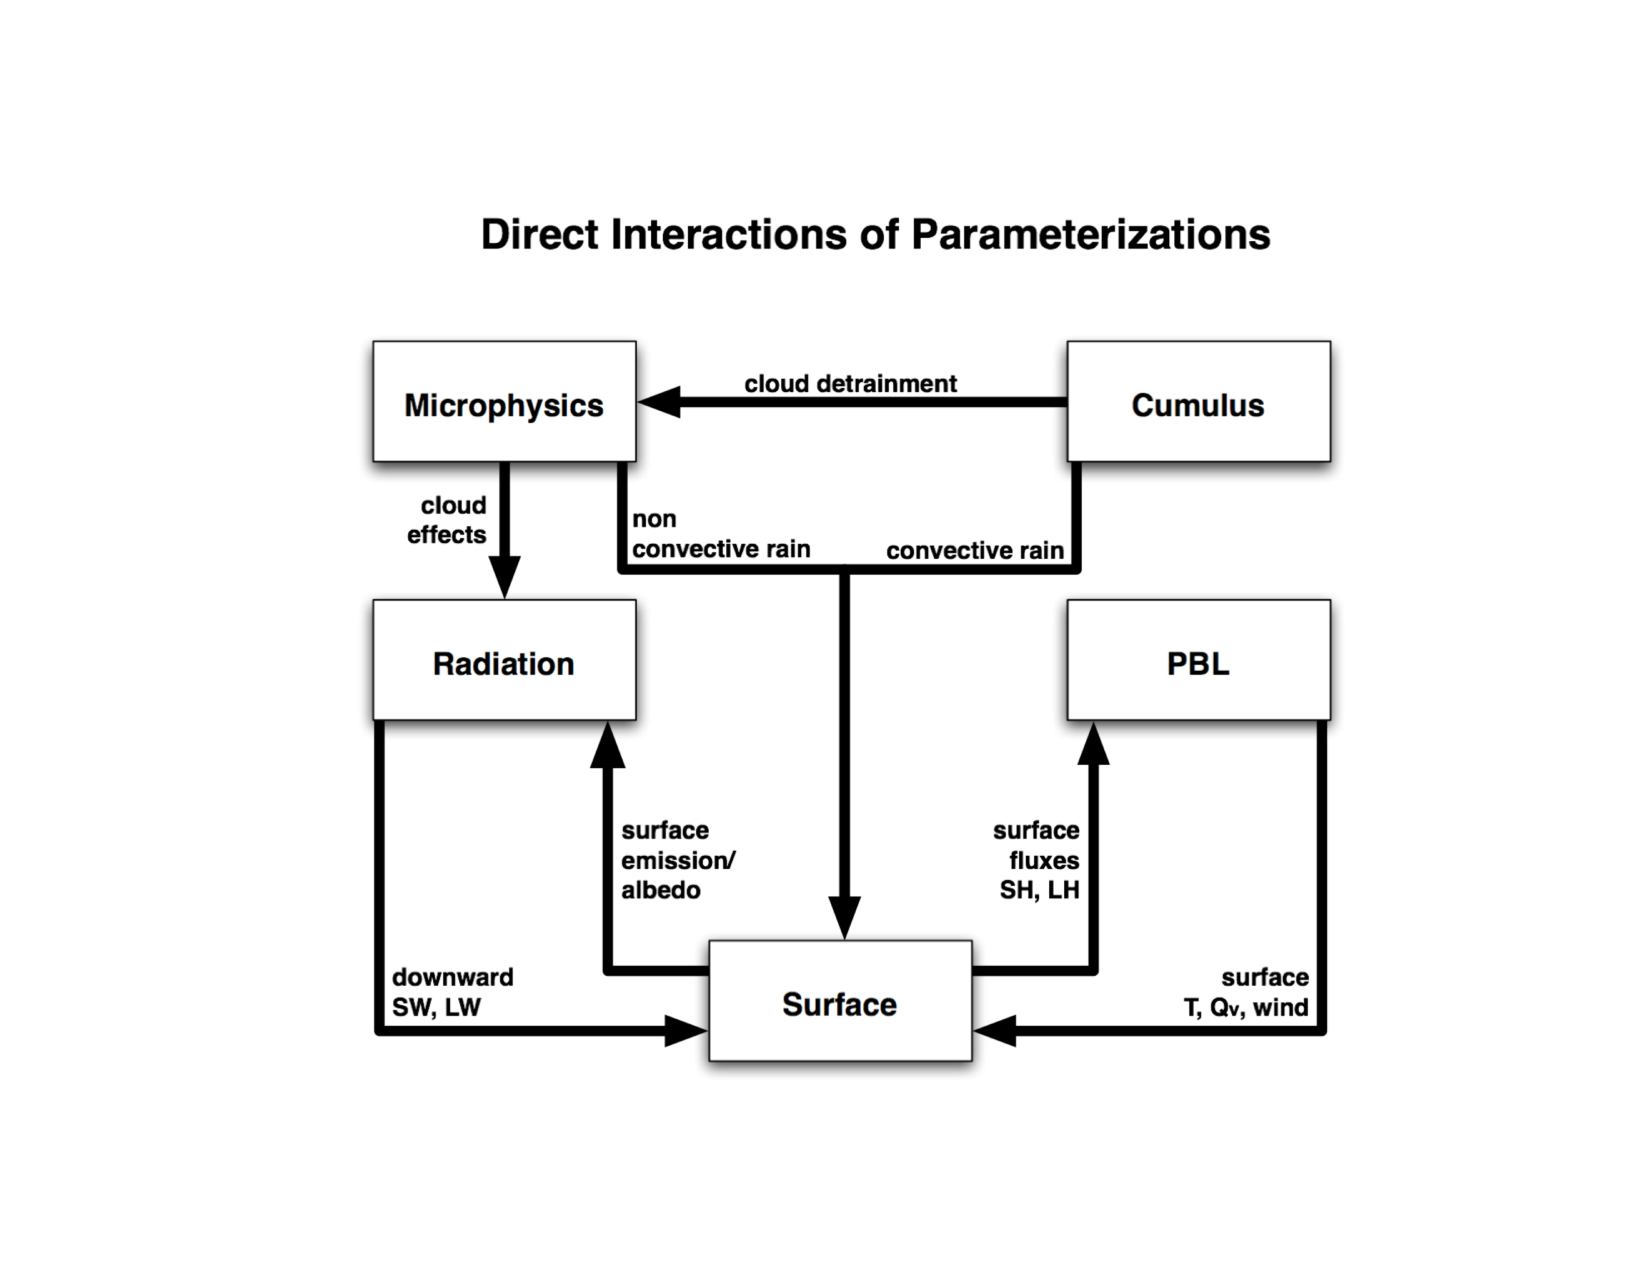
\includegraphics[width=4.0in]{figures/physics.pdf}
  \caption{\label{figure:physics}Diagram showing interactions between
   various physics components.}
\end{figure}

While the model physics parameterizations are categorized in a modular way,
it should be noted that there are many interactions between them via the
model state variables (potential temperature, moisture, wind, etc.)
and their tendencies, and via the surface fluxes, as shown in Fig.\ref{figure:physics}.
Table \ref {physics interaction table} summarizes how the various physics
processes interact in the model. In the table, {\em i} indicates that the 
state variable or flux is required input for the physics scheme, and {\em o}
indicates that the tendency or flux is a probable output of the scheme.
It can be seen that all the physical schemes interact in some way with the surface
physics (land-surface models, and, potentially, coupled ocean models).
The surface physics, while not explicitly producing tendencies of atmospheric
state variables, is responsible for updating the land-state variables.

\begin{table}
\caption{Physics Interactions. Columns correspond to
model physical processes: radiation (Rad),
microphysics (MP), cumulus parameterization (CP), planetary boundary layer/vertical diffusion
(PBL), and surface physics (Sfc). Rows corresponds to
model variables where {\em i} and {\em o} indicate whether a variable is
input or output (updated) by a physical process.}
\label{physics interaction table}
$$\vbox
{\halign{#\hfil \qquad & #\hfil \qquad & \hfil#\hfil \qquad & \hfil#\hfil
\qquad & \hfil#\hfil \qquad &  \hfil#\hfil \qquad & \hfil#\hfil \cr
\multispan7\hrulefill \cr
                &              & Rad       & MP           & CP           & PBL      &   Sfc   \cr
\multispan7\hrulefill \cr
Atmospheric     &  Momentum    &           &              &      io       &  io     &           \cr
State or        &  Pot. Temp.  &   io      &     io       &     io       &  io     &           \cr
Tendencies      &  Water Vapor &    i      &     io       &     io       &  io     &           \cr
                &  Cloud       &    i      &     io       &      o       &  io     &           \cr
                &  Precip      &    i      &     io       &      o       &         &           \cr
\multispan7\hrulefill \cr
Surface         &  Longwave Up &    i      &              &              &         &    o      \cr
Fluxes          &  Longwave Down &  o      &              &              &         &    i      \cr
                &  Shortwave Up &   i      &              &              &         &    o      \cr
                &  Shortwave Down & o      &              &              &         &    i      \cr
                &  Sfc Convective Rain &   &              &      o       &         &    i      \cr
                &  Sfc Resolved Rain &     &      o       &              &         &    i      \cr
                &  Heat Flux &             &              &              &   i     &    o      \cr
                &  Moisture Flux &         &              &              &   i     &    o      \cr
                &  Surface Stress &        &              &              &   i     &    o      \cr
\multispan7\hrulefill \cr
}}$$
\end{table}

Note also that, as mentioned, the microphysics does not output tendencies,
but updates the atmospheric state at the end of the model time-step. Unlike
for other physics, there is no option in ARW to call microphysics at lower
frequencies than the model time step mainly because of its important saturation
adjustment function that interacts with the dynamics especially in rseolved convection.
However, the rest of the {\em o}'s in the upper half of the table are
representative of the physical tendencies of these variables in the model.

The radiation, boundary-layer and cumulus parameterization schemes all
output tendencies, but the tendencies are not added until later in the solver where their
sum contributes to the forcing for the dynamics, so
from this perspective the order of call is not important. Moreover, these
physics schemes do not have to be called at the same frequency as each other
or the model time step. When lower frequencies are used, their tendencies
are kept constant between calls. This is typically done for the radiation schemes,
which are too expensive to call every timestep, and often for the cumulus schemes, for
which it may only be necessary to update the convective columns every five minutes or so. 
However, the surface/boundary-layer schemes are
normally called every step in ARW because this is likely to give the best results,
but the option is available to use a less frequent call that may be useful for the more
expensive CLM4 LSM.

The radiation is called first because of the required radiative fluxes
that are input to the land-surface scheme. The land-surface also requires rainfall
from the microphysics and cumulus schemes, but that is from the previous time-step
since it is called before the cumulus scheme and the microphysics is at the end of the time-step.
The boundary-layer scheme is necessarily after the land-surface scheme
because it requires the heat and moisture fluxes. Some cumulus schemes (Grell options)
also use the boundary-layer tendencies.

